\begin{figure}[H]
    \centering
    \caption{LRU priority queue of elements on the trace: A,B,C,B,A,D,C}
    \label{fig:my_label}
\newcounter{row}
\newcounter{col}

\newcommand\setrow[9]{
  \setcounter{col}{-3}
  \foreach \n in {#1, #2, #3, #4, #5, #6, #7, #8, #9} {
    \edef\x{\value{col} - 0.4}
    \edef\y{5.5 - \value{row}}
    \node[anchor=center] at (\x, \y) {\n};
    \stepcounter{col}
  }
  \stepcounter{row}
}

\newcommand\setrows[9]{
  \setcounter{col}{-1}
  \foreach \n in {#1, #2, #3, #4, #5, #6, #7, #8, #9} {
    \edef\x{\value{col} - 0.4}
    \edef\y{5.5 - \value{row}}
    \node[anchor=center] at (\x, \y) {\n};
    \stepcounter{col}
  }
  \stepcounter{row}
}
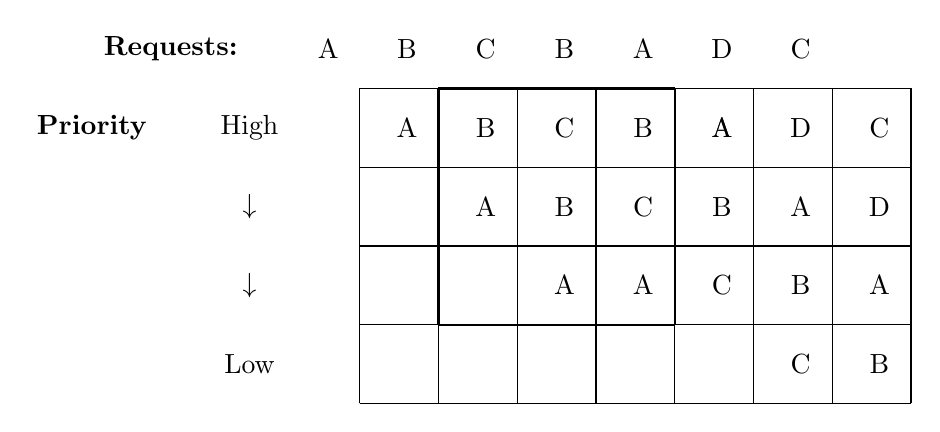
\begin{tikzpicture}[scale=1]

\begin{scope}
\draw (0, 0) grid (7, 4);
\draw[very thin] (0, 0) grid (7, 4);
\draw[thick,-] (1,1) -- (4,1);
\draw[thick,-] (1,1) -- (1,4);
\draw[thick](1,4) --(4,4);
\draw[thick](4,1) --(4,4);
\setcounter{row}{1}
\setrow {}{\textbf{Requests:}}{}{A}{B}{C}{B}{A}{D}
\setrow {\textbf{Priority}}{}{High}{}{A}{B}{C}{B}{A}
\setrow {}{}{$\downarrow$}{ }{}{}{}{}{}
\setrow {}{}{$\downarrow$}{ }{}{}{}{}{}
\setrow {}{}{Low}{}{}{}{}{}{}

\end{scope}
\begin{scope}
\setcounter{row}{1}
\setrows {}{}{}{}{}{}{}{C}{}
\setrows {}{}{}{}{}{}{A}{D}{C}
\setrows {}{}{}{A}{B}{C}{B}{A}{D}
\setrows {}{}{}{}{A}{A}{C}{B}{A}
\setrows {}{}{}{}{}{}{}{C}{B}
\end{scope}
\end{tikzpicture}
\end{figure}